\chapter{Results of Workflow Validation}\label{chap:results}
The Galaxy workflows are validated using real-world datasets from different laboratories. The analysis results for each workflow with complying test samples are described below.

\section{Poxvirus Workflow with Lumpy Skin Disease Virus Datasets}
We employed our pipeline using a tiling amplicon approach with masked reference sequences for each half genome to ensure an unambiguous mapping to the identical two \ac{ITR} regions of the poxvirus genome. Two public \ac{LSDV} samples, 20L70 (MZ577075.1) and 20L81 (MZ577076.1), that were sequenced using a primer scheme with two primer pools are used and retrieved from GenBank on 10\textsuperscript{th} April, 2023. Collected from cattle in 2020 during a lumpy skin disease outbreak in Northern Vietnam (20L70\_Dinh-To/VNM/20 and 20L81\_Bang-Thanh/VNM/20), both samples were sequenced on a MiSeq System using a Nextera XT library preparation kit. \\
The used \acs{CaPV} primer scheme in \ac{BED} format contains information about the primer pairs used for the amplicons. Each primer pair has one positive and one negative strand primer, indicated by the strand in the sixth column and by the \textit{LEFT} and \textit{RIGHT} label in the name. Primers are labeled in an alternating way: \textit{pool1} primer pairs are denoted as \textit{pool1a} and \textit{pool1b}. We use the same method for \textit{pool2} with \textit{pool2a} and \textit{pool2b}. We reuse the \textit{SCORE} column from the \ac{BED} file to unambiguously identify primer and strand for each amplicon. The annotated primer scheme for \ac{CaPV} is part of the workflow run to which links are provided in Supplementary~\secref{sec:apx-aiv-links}. The \ac{LSDV} ``Neethling'' strain was used as reference genome (NC\_003027.1, retrieved on GenBank 10\textsuperscript{th} April, 2023) for mapping. The raw FASTQ files for each sample were quality trimmed with \texttt{fastp} and mapped to each half-masked reference, which is explained in detail below. Preprocessing with default \texttt{fastp} settings includes automatically detected adapter trimming, a quality filter to discard reads below an average quality of Q15, with more than 5 uncalled (N) bases and 40\% unqualified bases, a length filter to discard reads below a threshold of 30, automatic trimming of polyG tails for Illumina NextSeq/NovaSeq data and a minimum length of 10 to detect polyG tails.
\\
% downstream: gene expression analysis, variant calling

\setlength{\tabcolsep}{16pt}
\renewcommand{\arraystretch}{1.3}
\begin{table}[ht!]
    \centering
    \begin{tabular}{lcc}
    \toprule
    \textbf{Output Metric}                      & \textbf{20L70}     & \textbf{20L81}     \\ \midrule
    Paired-end raw reads                        & 863 820            & 1 016 168          \\ 
    Paired-end reads after quality trimming     & 856 138            & 947 064            \\ \midrule
    Proportion of reads mapping to reference    & 99.6\%             & 77.3\%             \\ 
    Proportion of reference covered             & 99.68\%            & 99.68\%            \\ \midrule
    Mean coverage                               & 2 705.2\texttimes & 2 411.4\texttimes \\ 
    Alignment error rate                        & 1.25\%             & 1.30\%             \\ \bottomrule
    \end{tabular}
    \caption{Metrics after preprocessing and mapping for datasets 20L70 and 20L81.}
    \label{tab:4-pox-metrics}
\end{table}

\begin{figure}[ht!]
    \centering
    \hspace*{-8pt}
    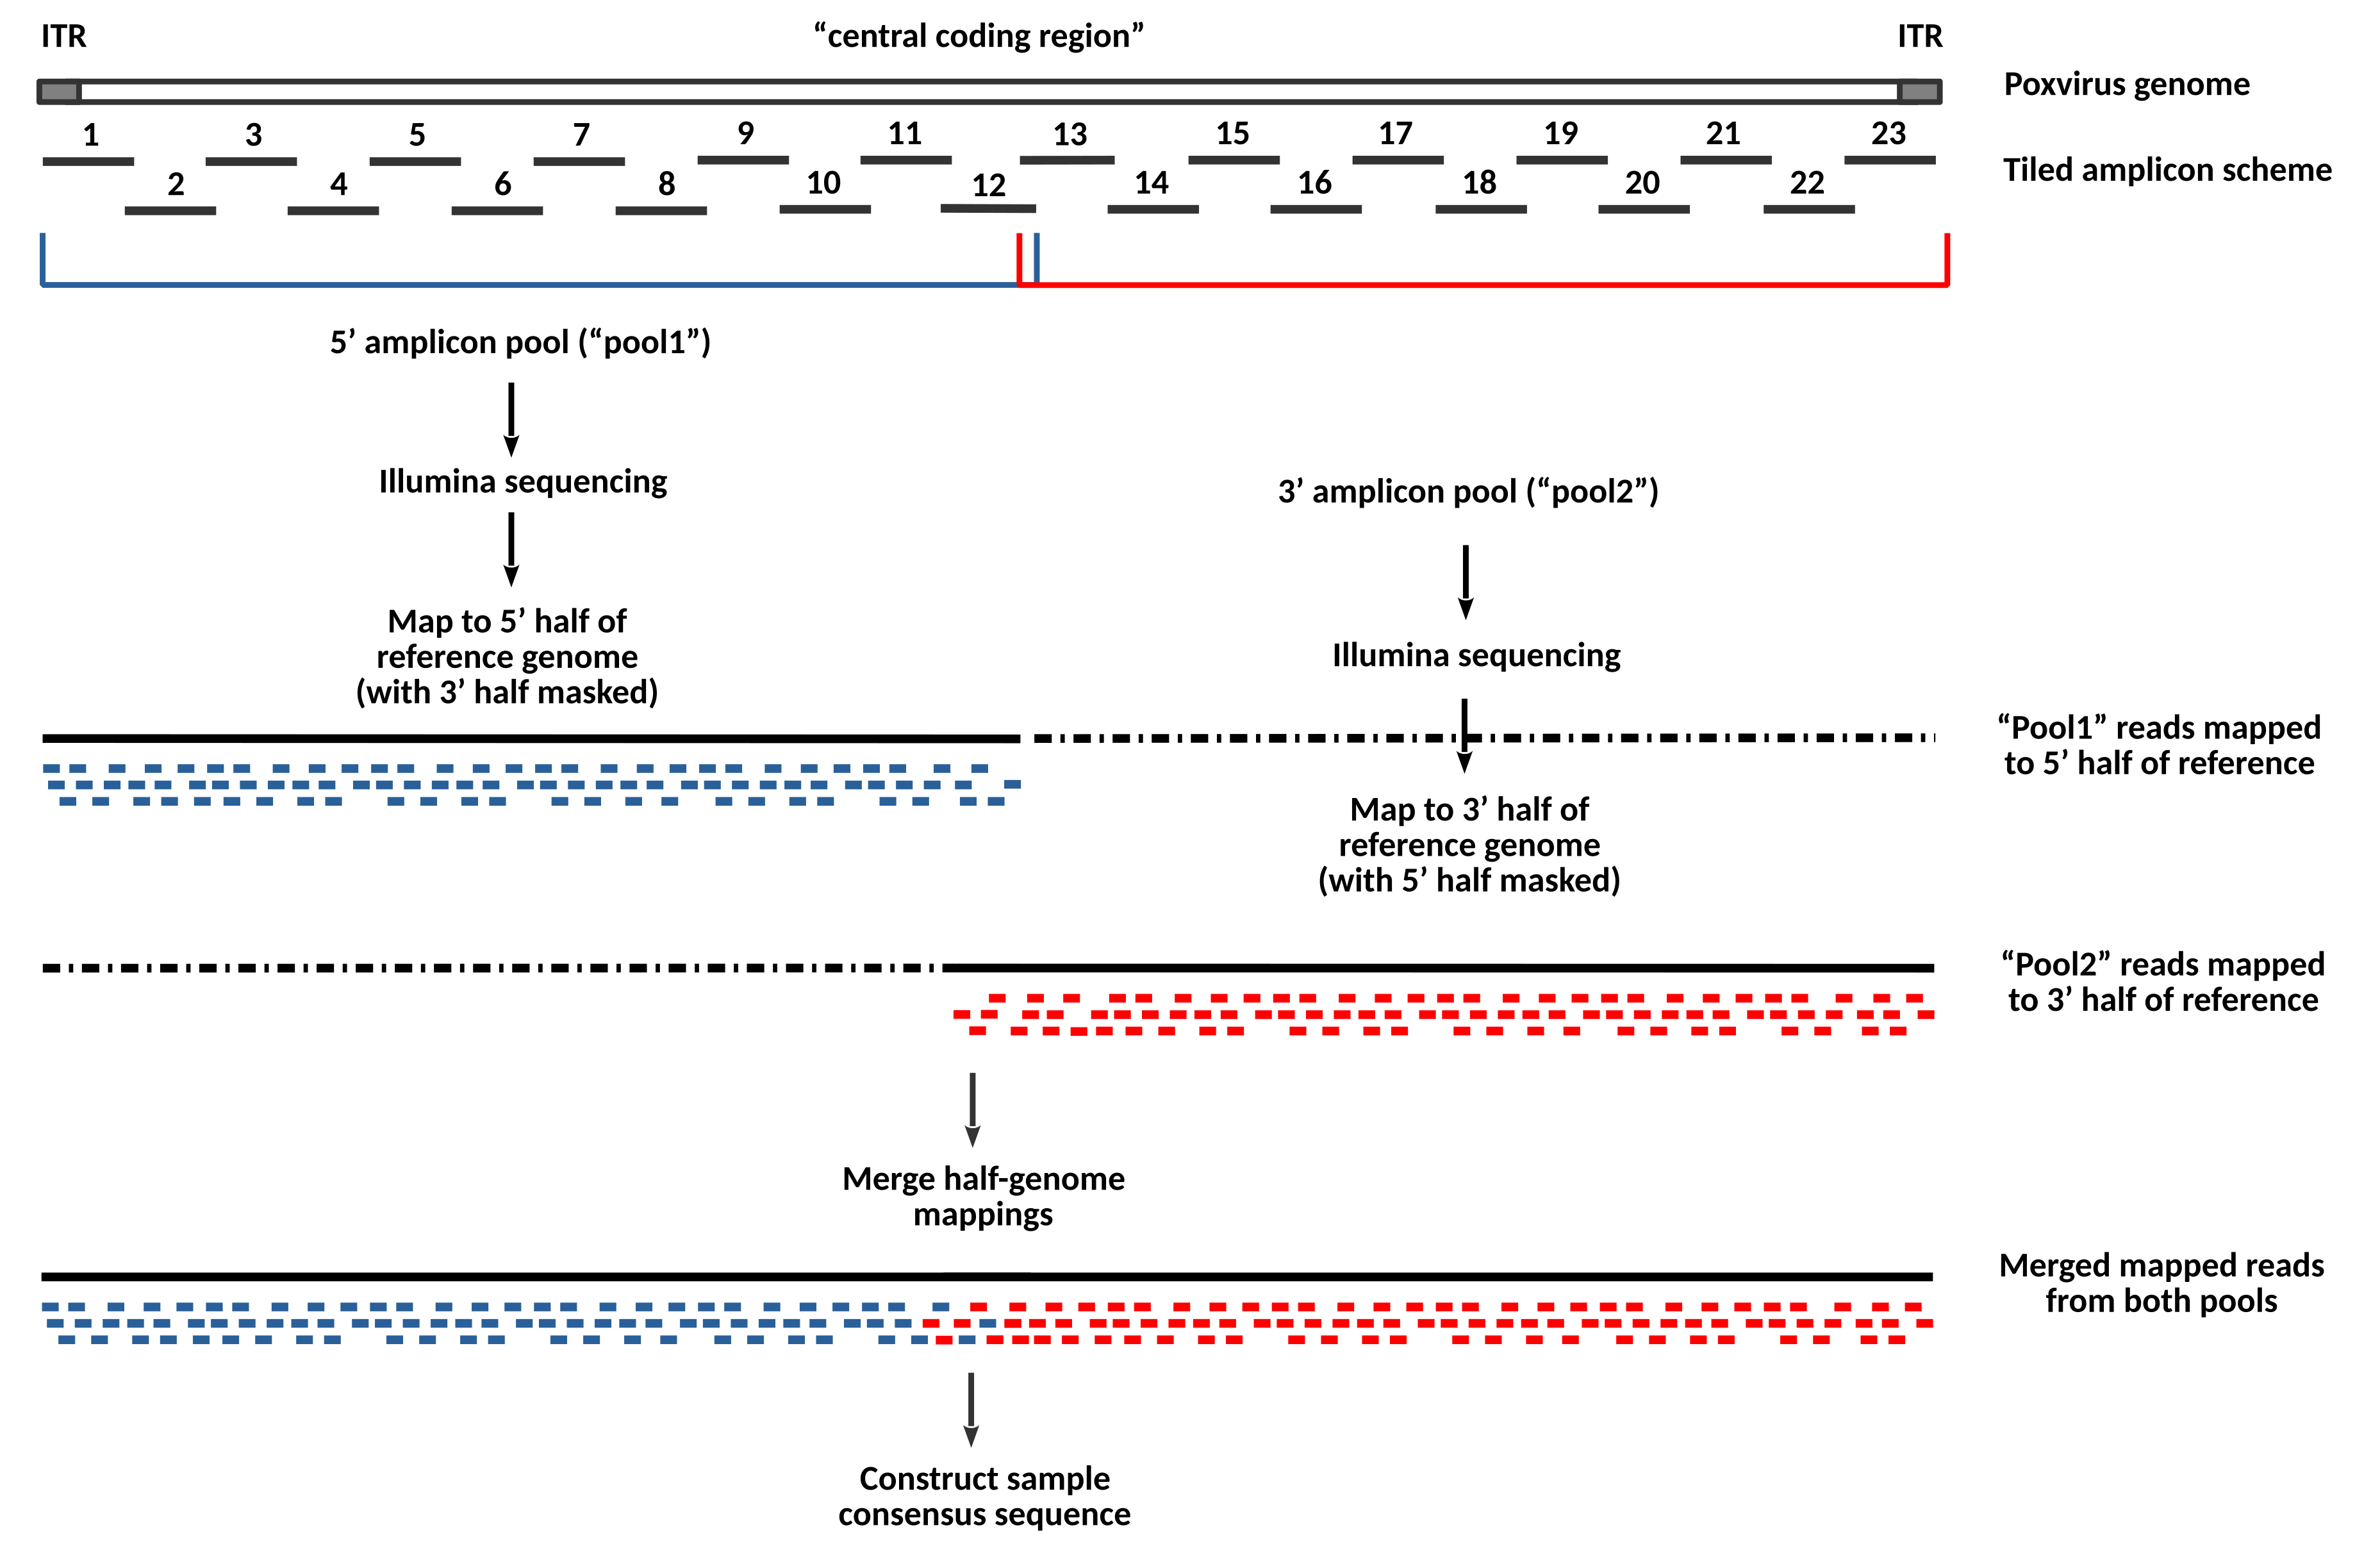
\includegraphics[width=1.1\textwidth]{media/4-pox-ampl-fig.png}
    \caption[Tiling amplicon scheme used in poxvirus workflow.]{Tiling amplicon scheme emphasising masking of the reference, mapping in two pools and merging of mappings with almost no overlap.}
    \label{fig:4-pox-ampl}
\end{figure}
The used primer scheme contains a total of 23 primers, while the first set of 12 primers covers the 5' genome end labeled with \textit{pool1}, and the remaining 11 primers cover the 3' genome end, labeled with \textit{pool2} as depicted at the top in blue (\textit{pool1}) and red (\textit{pool2}) in~\figref{fig:4-pox-ampl}. This scheme was designed for the tiling amplicon approach and allows to generate the complete genome of all three members of Capripoxviruses, which includes the \ac{LSDV} sample. %The primer scheme works with all Capripoxviruses due to the serological similarity they have.
The primer scheme is provided in the Galaxy history of the test runs and is available via links in Supplementary~\secref{sec:apx-pox-links}. Inspection  of the masking intervals for N-masking the reference confirms that the right-most position of Ns of masking the 5' half (i.e. preparing the reference for mapping \textit{pool2} reads) is the minimal start position of \textit{pool2} primers (``1 -- 79081'', and 79081 being the start position of primer 13). Accordingly for N-masking the reference for mapping of \textit{pool1} reads, the position of the right-most primer end of \textit{pool1} primers (primer 12) is 80202, resulting in the interval ``80202 -- 150773''. This is clearly visible in~\figref{fig:4-lsdv-read-groups}, where reads from \textit{pool1} are labeled in red and \textit{pool2} in blue, and mapped to the same reference sequence with different masked parts. \\ % coverage is depicted and as expected higher - mapping from both pools
The final position is the maximal end position and the total length of the reference sequence. Since the reference genome and primer scheme are the same for both datasets 20L70 and 20L81, the N-masked references are used for both mappings. Mapping of each pool is done with \texttt{BWA-MEM} and default settings for Illumina-sequenced reads, using the N-masked reference for \textit{pool1} and \textit{pool2} respectively. This results in a mapping with a small overlap in the central part of the genome, where primer 12 ends and primer 13 starts as indicated in the top of~\figref{fig:4-pox-ampl}. After merging the mappings with \texttt{Samtools merge}, statistics for preprocessing and mapping are reported and summarised in~\tabref{tab:4-pox-metrics}. \figref{fig:4-lsdv-read-groups} shows a screenshot from \ac{IGV}, where the mapping of reads from \textit{pool1} (red) and \textit{pool2} (blue) are merged and demonstrate a higher coverage in the overlapping part of the reference sequence which was mapped to in both pools. For both samples 20L70 and 20L81, almost the complete reference genome was covered during mapping (99.68\%) with a mean coverage of {2705.2\texttimes } and {2411.4\texttimes } respectively. Primer end positions of \textit{pool2} primers are highlighted with blue circles and mark the start position of the overlapping region and the end of the masking of the reference sequence for \textit{pool2}.
\\

\begin{figure}[ht!]
    \centering
    \hspace*{-24pt}
    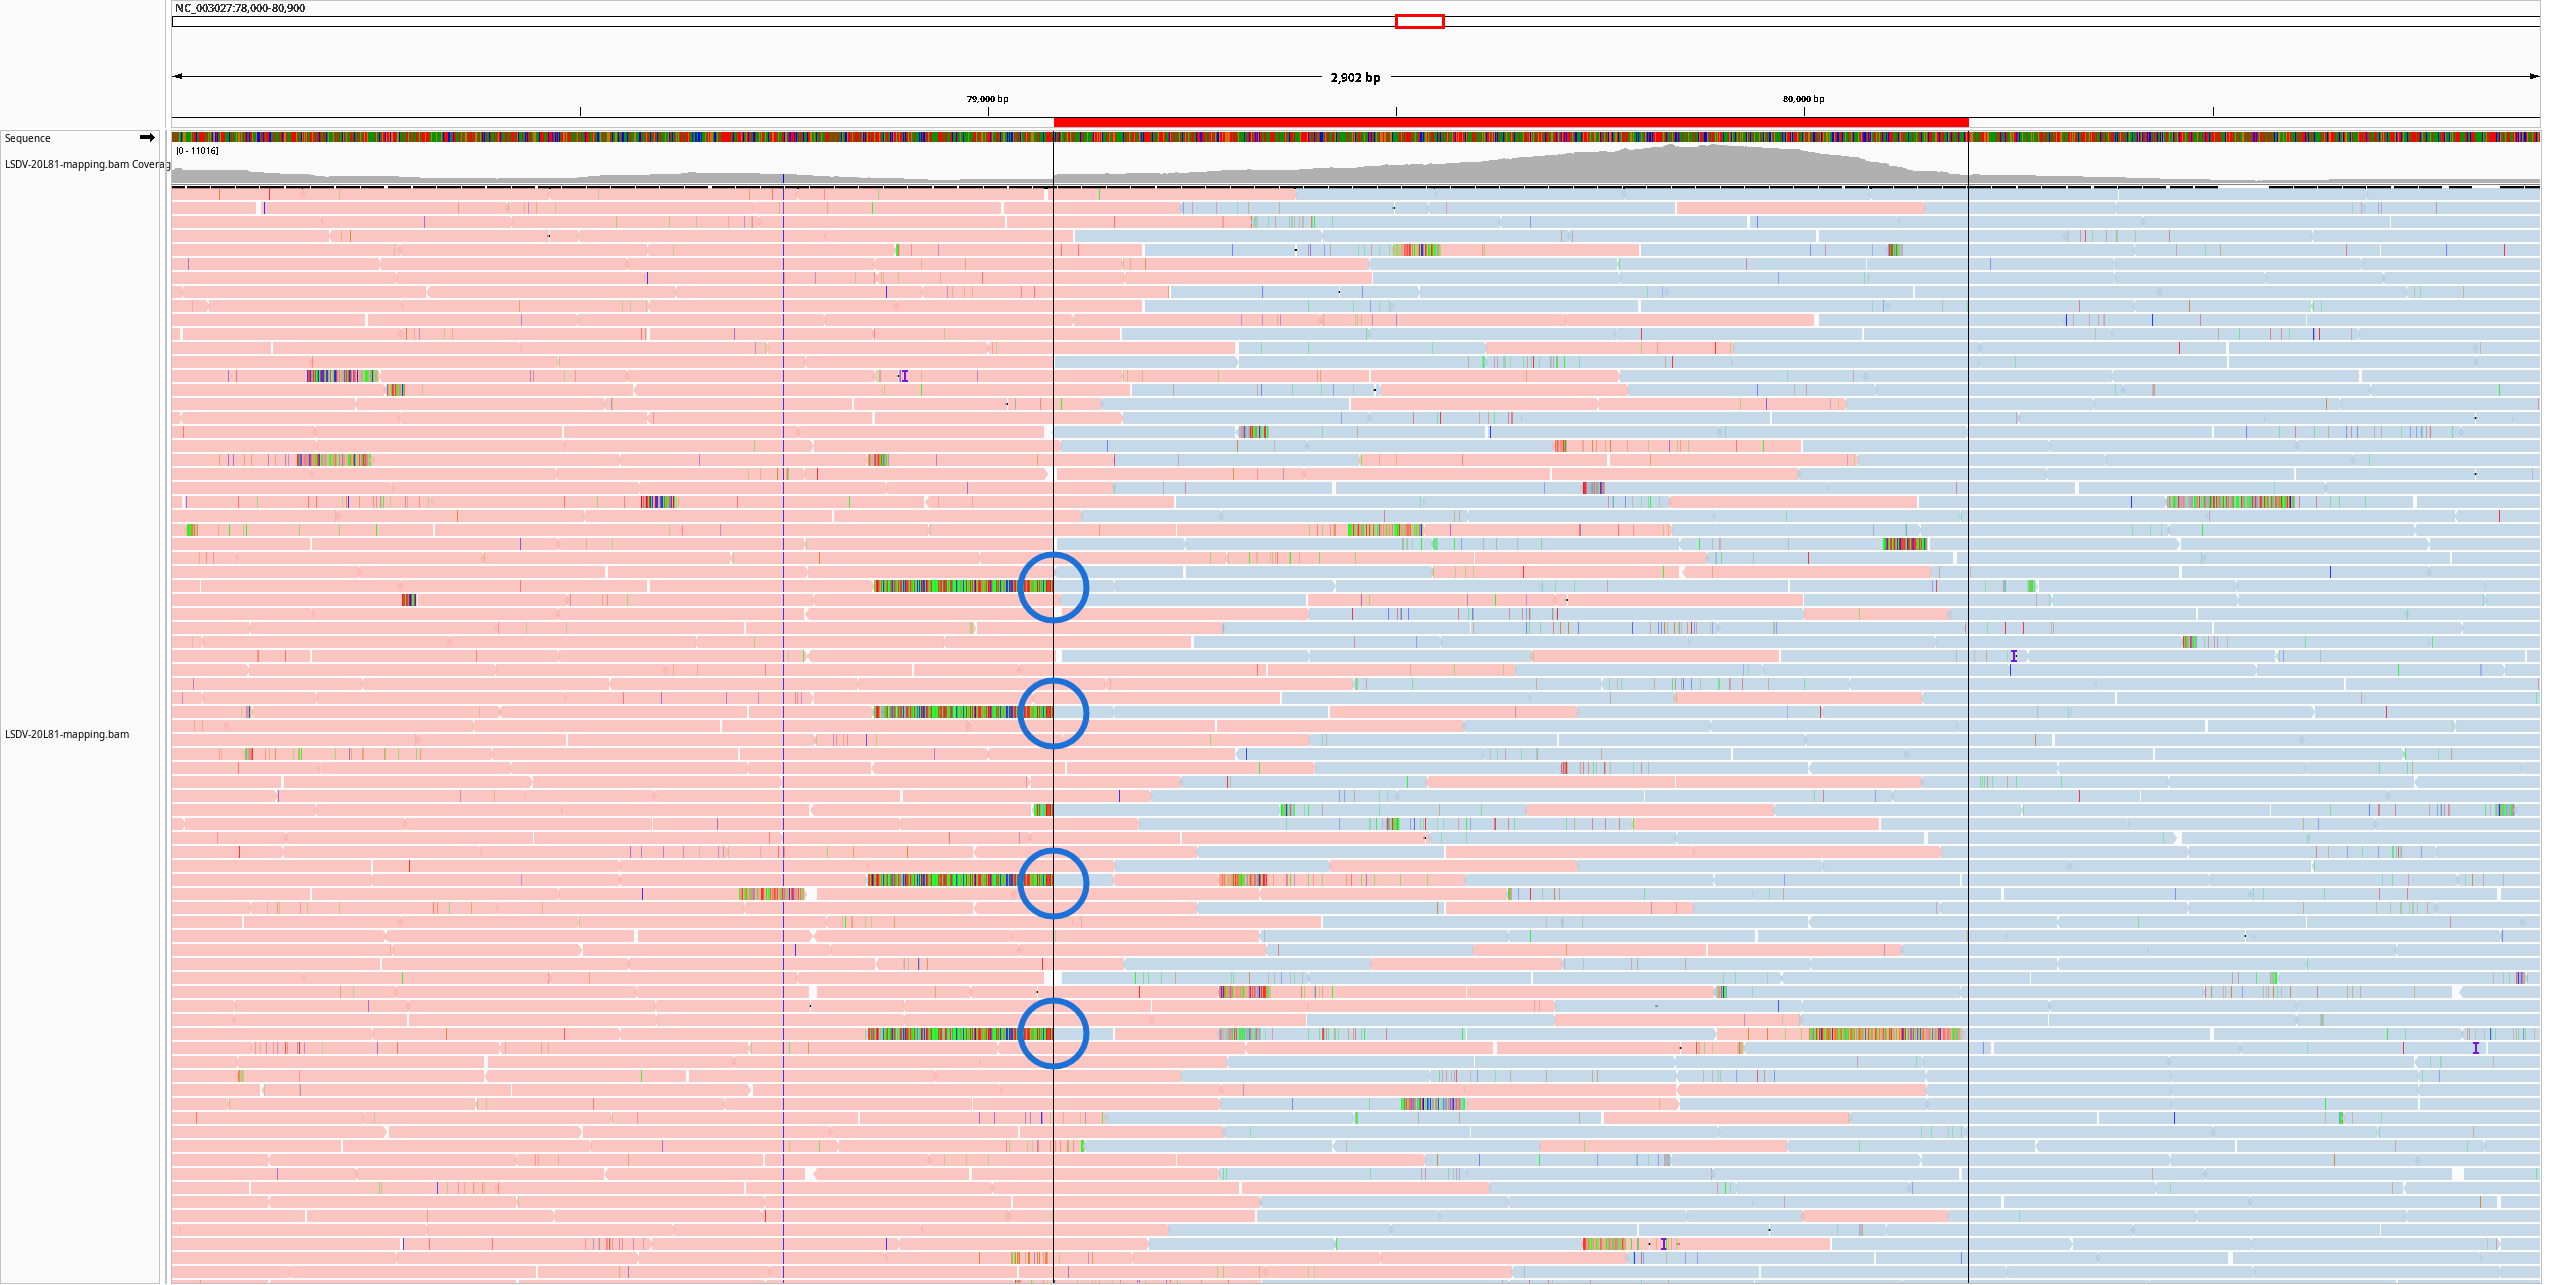
\includegraphics[width=1.1\textwidth]{media/4-lsdv-alig-20L81-c.png}
    \caption[Overlapping reads region of LSDV mapping in 20L81 sample.]{Overlapping, seamlessly merged mapping region of the two amplicon pools of the 20L81 sample. Coloured reads indicate read groups from \textit{pool1} (red) and \textit{pool2} (blue), primers are soft-clipped and end where the mapping of \textit{pool2} reads starts, as marked with blue circles for primer 13 to which four reads from \textit{pool2} bind. More primers may bind outside of the cropped snapshot.}
    \label{fig:4-lsdv-read-groups}
\end{figure}

The merged mapping of both read pools was quality trimmed with \texttt{iVar trim} to remove primers and reads with a length of less than 30 bp. The remaining reads were used for full-length consensus sequence construction with \textit{iVar consensus}, developed for amplicon-based sequencing data. Inspection of the consensus sequences for both samples shows that apart from low coverage regions in the 5' front and 3' tail due to ampliconic sequencing, a consensus sequence was produced and a base at each position could be found. A base could not be called in the consensus at the first 264 positions in both the 20L70 and 20L81 sample, which corresponds to the primer binding site on the forward strand, and no bases at the last 268 positions indicate the remaining part where the last primer on the reverse strand starts. This is expected due to coverage criteria outside of the amplicons that were not met in these regions.\\
%  This indicates that the hosts were vaccinated with the concerned vaccine Lumpivax, what suggests that the resulting recombinant genome can be reliably mapped to other viruses belonging to the Capripoxvirus family.
Recent research revealed the presence of non-Neethling strains in samples from recombinant vaccine-like \ac{LSDV} genomes, and the two testing samples are shown to be from this recombinant strain~\cite{vandenbussche2022recombinant}. Mapping the \ac{LSDV} reads to the Neethling strain, the recommended reference genome for \ac{LSDV}, seems a viable approach for base-by-base consensus generation as shown. However, the 20L70 and 20L81 samples are subject to a research that revealed the presence of other \ac{CaPV} strains in a Neethling-based vaccine and also stating the infected animals from the samples being recombinant strains that resemble this \ac{LSDV}-like vaccine~\cite{vandenbussche2022recombinant}. Therefore, we validated this experiment by running the poxvirus workflow with reference sequences from the other two \ac{CaPV} members, \ac{SPPV} (NC\_004002.1) and \ac{GTPV} (NC\_004003.1). Using the \ac{CaPV} primer scheme with the 20L70 and 20L81 samples, the generated consensus sequences for \ac{SPPV} and \ac{GTPV} respectively obtain highly similar consensus sequences as with the Neethling strain reference. Due to unadapted primer binding sites for \ac{SPPV} and \ac{GTPV}, coverage in both ends of the consensus sequences dropped to below the consensus coverage threshold. Otherwise, comparing the amount of \acp{SNP} that each of the \ac{LSDV}-, \ac{SPPV}- and \ac{GTPV}-based consensus sequences have relative to each reference sequence, high similarities among the consensus sequences are found. \tabref{tab:pox-capv-ref} lists the exact numbers of \acp{SNP} per consensus sequence generated from each the 20L70 and 20L81 samples. While all genes of \ac{SPPV} and \ac{GTPV} are present in the \ac{LSDV} genome and sharing a sequence identity of 97\%, there are 9 genes from \ac{LSDV} that are disrupted in both \ac{SPPV} and \ac{GTPV} genomes~\cite{tulman2002genomes}. These small differences and similarities are reflected in the number of \acp{SNP} present, relative to each of the \ac{CaPV} reference sequences. The consensus sequence generated by mapped reads to the \ac{GTPV} reference has the fewest \acp{SNP} relative to the \ac{SPPV} reference (32 080 in sample 20L70 and 32 177 in sample 20L81), and vice versa the \ac{SPPV}-mapped consensus sequence has the fewest \acp{SNP} compared to the \ac{GTPV} reference sequence (28 623 in sample 20L70 and 28 663 in sample 20L81), indicating the high similarities among \ac{SPPV} and \ac{GTPV}. Compared to the Neethling strain, the \ac{SPPV}-mapped consensus sequence has the fewest \acp{SNP} (8 506 in sample 20L70 and 8 505 in sample 20L81). The difference to the amount of \acp{SNP} of the \ac{LSDV}-based consensus sequence is very small and overall accounts for the high mutation rate of Capripoxviruses.
\\

\setlength{\tabcolsep}{8pt}
\renewcommand{\arraystretch}{1.3}
\begin{table}[ht!]
    \centering
    \begin{tabular}{@{}cccc@{}}
    \toprule
    \multirow{2}{*}{\textbf{\begin{tabular}[c]{@{}c@{}}Consensus sequence\\ based on ref. \textsuperscript{1}\end{tabular}}} & \multirow{2}{*}{\textbf{SNPs relative to}}                                                 & \multicolumn{2}{c}{\textbf{\# of SNPs}}       \\ \cmidrule(l){3-4} 
                                                                                                                           &                                                                                            & \textbf{20L70 sample} & \textbf{20L81 sample} \\ \midrule
    LSDV                                                                                                                   & \multirow{3}{*}{\begin{tabular}[c]{@{}c@{}}NC\_003027.1\\ (Neethling strain)\end{tabular}} & 8 619                 & 8 610                 \\
    SPPV                                                                                                                   &                                                                                            & 8 506                 & 8 505                 \\
    GTPV                                                                                                                   &                                                                                            & 8 619                 & 8 544                 \\ \midrule
    LSDV                                                                                                                   & \multirow{3}{*}{\begin{tabular}[c]{@{}c@{}}NC\_004002.1\\ (SPPV reference)\end{tabular}}   & 32 341                & 32 373                \\
    SPPV                                                                                                                   &                                                                                            & 32 310                & 32 321                \\
    GTPV                                                                                                                   &                                                                                            & 32 080                & 32 177                \\ \midrule
    LSDV                                                                                                                   & \multirow{3}{*}{\begin{tabular}[c]{@{}c@{}}NC\_004003.1\\ (GTPV reference)\end{tabular}}   & 28 822                & 28 844                \\
    SPPV                                                                                                                   &                                                                                            & 28 623                & 28 663                \\
    GTPV                                                                                                                   &                                                                                            & 28 683                & 28 766                \\ \bottomrule
    \multicolumn{4}{l}{\begin{tabular}[c]{@{}l@{}}\textsuperscript{1} Consensus sequences generated by mapping the same preprocessed reads to the\\ respective reference.\\\end{tabular}}                                                
    \end{tabular}
    \caption[Comparison of amount of SNPs of CaPV consensus sequences.]{Comparison of amount of SNPs of CaPV consensus sequences relative to each of the CaPV reference sequences. Consensus sequences were generated using the poxvirus workflow with the 20L70 and 20L81 sample, CaPV primer scheme and the mentioned reference sequence for mapping.}
\label{tab:pox-capv-ref}
\end{table}

\section{AIV Workflow with H4N6 and H5N8 Samples}\label{sec:4-aiv}
\setlength{\tabcolsep}{14pt}
\renewcommand{\arraystretch}{1.3}
\begin{table}[ht!]
    \centering
    \begin{tabular}{lcc} 
    \toprule
    \textbf{Output Metric}                                                                & \textbf{H4N6} & \textbf{H5N8} \\ \midrule
    Paired-end raw reads                                                                  & 1 537 722                  & 858 610                    \\ 
    \begin{tabular}[c]{@{}l@{}}Paired-end reads after quality\\trimming\end{tabular}      & 1 507 396                  & 830 176                    \\ \bottomrule
    \end{tabular}
    \caption[Metrics after preprocessing of H4N6 and H5N8 samples.]{Metrics about Illumina reads before and after preprocessing of H4N6 and H5N8 samples.}
    \label{tab:4-aiv-metrics}
\end{table}

The \ac{AIV} Illumina workflow on the Galaxy platform was evaluated using two field isolates provided by Sciensano, the Belgian national health institute. The isolates were extracted in Belgium in 2020 from an H4N6 infected magpie (EPI\_ISL\_7593059) and an H5N8 infected duck (EPI\_ISL\_7596571). For reasons of readability, we refer to the samples as H4N6 and H5N8 samples. The two samples were sequenced on an Illumina platform in paired-end mode and are utilised one sample per workflow run on Galaxy. For the \ac{AIV} Illumina workflow, a reference database in FASTA format is required as a collection, i.e. a list of one dataset per \ac{AIV} segment, which is uploaded in Galaxy. The used database contains multiple sequences per segment as described in~\secref{sec:3-aiv-ref}. The amount of sequences and distribution of subtypes within each segments suggests that variation within each subtype is generally captured well with the given database. Due to the filtering criteria, not all eight segments of one sample were found suitable for the database.\\
After starting the workflow, the paired-end reads were preprocessed and serve as query reads for \texttt{VAPOR}. Metrics of before and after preprocessing are shown in~\tabref{tab:4-aiv-metrics} and count more than 1.50 million reads after preprocessing for the H4N6 sample and 0.83 million reads for the H5N8 dataset. Since the reference database contains eight FASTA files in a collection, \texttt{VAPOR} runs once per dataset and outputs the highest scoring sequences per segment, which represents the most similar sequences from the database compared to the query sequences. \\

\setlength{\tabcolsep}{8pt}
\renewcommand{\arraystretch}{1.3}
\begin{table}[ht!]
    \centering
    \hspace*{-16pt}
    \begin{tabular}{@{}lcccc@{}}
    \toprule
    \multicolumn{1}{l}{\textbf{Segment}} & \multicolumn{2}{c}{\textbf{Proportion of query bases in reads}}                             & \multicolumn{2}{c}{\textbf{AIV subtype of hit}}                                         \\ \midrule
                                         & \multicolumn{1}{l}{\textbf{H4N6 sample}} & \multicolumn{1}{l}{\textbf{H5N8 sample}} & \multicolumn{1}{l}{\textbf{H4N6 sample}} & \multicolumn{1}{l}{\textbf{H5N8 sample}} \\ \cmidrule(l){2-5} 
    HA                                   & 98.7\%                                    & 100.\%0                                      & H4                                       & H5                                       \\
    NA                                   & 98.7\%                                    & 100.0\%                                      & N6                                       & N8                                       \\ \bottomrule
    \end{tabular}
    \caption[Results of VAPOR run with AIV test samples.]{The best scoring sequence of the VAPOR run for each AIV test samples, indicating a perfect match (100\% of the query bases are in the reads) of the HA and NA segments of the H5N8 sample sequence, and almost all query bases of the H4N6 sample in the found sample.}    
\label{tab:4-aiv-vapor}
\end{table}

The \texttt{VAPOR} search was able to successfully identify the avian influenza virus subtypes present in each sample: for the H5N8 sample, the most similar sequence of HA segment origins from a sample with the H5 subtype, while the most similar sequence of the NA segment origins from a sample with the N8 subtype. Both found gene sequences contain 100\% of the input reads. Similarly, the H4N6 sample was correctly identified with concordance of query bases of 98.7\%. The results of the \texttt{VAPOR} run for the HA and NA genes are summarised in~\tabref{tab:4-aiv-vapor}. \\
Consensus sequences for each segment were constructed with \texttt{iVar consensus} and while a consensus could be found for each position, they are 100\% identical to the originally assembled reads that were uploaded to \ac{GISAID} by Sciensano from the same sample. Due to slightly different genome sizes of the reference sequence used for mapping compared to the assembly, the resulting consensus sequences in the \ac{AIV} workflow are shorter than the assembled sequences on \ac{GISAID}. The consensus sequence for the \ac{HA} segment of the H4N6 sample is differing in 1 bp in the 5' end, and 4 bp in the 3' end. The consensus sequence constructed for the \ac{NA} gene misses 18 bp compared to the assembled sequence on \ac{GISAID} in the 5' end and 33 bp in the 3' end. Similarily, the \ac{HA} consensus sequence of sample H5N8 is 28 bp shorter in the front and 44 bp shorter in the end. The \ac{NA} consensus sequence differs in 20 and 28 bp in the front and tail. These differences in length can occur due to different reference sequence lengths, consensus coverage thresholds or different preprocessing settings. \\
Other workflow outputs for the \ac{AIV} samples include plots that visually emphasise \acp{SNP} relative to the top hits of the \texttt{VAPOR} run, indicating the most similar sequences from the reference collection. The plots for the \ac{HA} and \ac{NA} genes for the H4N6 sample (\figref{fig:apx-aiv-snipit-s4}) show 30 \acp{SNP} compared to the first sequence which was also used as reference for mapping (LC121412.1) and 31 \acp{SNP} compared to the second best result (MK192399.1). Similarly, the \ac{NA} gene consensus sequence has 29 \acp{SNP} compared to the reference sequence (MW19994.1). For the H5N8 sample, the \texttt{VAPOR} run found a sequence with 100\% of the query bases in the reads, and therefore the number of \acp{SNP} is expected to be low. Supplementary~\figref{fig:apx-aiv-snipit-s8} shows there is one \ac{SNP} in the \ac{HA} gene compared to the reference (MZ166252.1) at position 1002 and one \ac{SNP} at position 497 compared to the \ac{NA} reference sequence (MZ166270.1). The \acp{SNP} indicate point mutations or mapping errors, low coverage or close calls during consensus sequence construction. \\
A protein FASTA file containing gene annotations is generated based on the consensus sequence with \texttt{Prokka} and can be used for detailed gene expression analysis. \\
Phylogenetic classification relative to the 30 most similar sequences in the \ac{AIV} reference database, queried by \texttt{VAPOR}, is done for each segment to reveal temporal and geographical relations of the isolate. Generated phylogenetic trees with \texttt{IQ-Tree} are depicted in Supplementary Figures~\ref{fig:apx-aiv-trees-s4} and~\ref{fig:apx-aiv-trees-s8}. The trees are unrooted and for the \ac{HA} gene of the H4N6 sample, shows the nearest clade being from an isolate which is a H4N6 infected mallard from the Netherlands, taken in 2017, and for the \ac{NA} a single and very early split is made where the gene is clustered to a H6N6 infected duck from Hunan, China. The obtained results for the H5N8 sample show clustering of both the \ac{HA} and \ac{NA} genes with sequences from a H5N8 infected mule duck from France, taken in 2020 and 2021.\\
Users of the workflow with real-world samples could investigate in more detail by uploading their own reference collection and hereby finding links to other sequenced samples from previous outbreaks in their region. The depth of the split in a phylogenetic tree can indicate the degree of relatedness between the sample and the other samples within that split. A deeper split suggests a closer relationship between the sample and the other samples in that particular branch.

\section{FMDV Workflows with Asia-1, A, SAT-1 and SAT-2 Samples}
The samples used for workflow validation are downloaded from the \ac{NCBI} and were chosen exemplatory for four of the seven different \ac{FMDV} serotypes. All four samples were sequenced on an Illumina NextSeq 550 platform. Two samples (Asia-1 serotype, SRR17960053 and A serotype, SRR18751245) were taken from infected cattle and buffalo during an outbreak in Pakistan from 2008 to 2012. One sample (SAT-1 serotype, SRR18685689) was isolated from buffaloes in Kenya in 2016 and plaque purified before sequencing, and the fourth sample (SAT-2 serotype, SRR9328470) was taken from an \ac{FMD} outbreak in Nigeria in 2014. \\
The results of before and after preprocessing of the raw reads are described in~\tabref{tab:4-fmdv-metrics}. The SAT-2 sample contains a very low number of reads with only 11 576 reads after preprocessing, however to show the ability of the developed workflows, it was kept in the test sample collection. 
\\

\setlength{\tabcolsep}{12pt}
\renewcommand{\arraystretch}{1.3}
\begin{table}[ht!]
    \centering
    \begin{tabular}{lcccc} 
    \toprule
    \textbf{Output Metric}                                                              & \textbf{Asia-1} & \textbf{A}                                           & \textbf{SAT-1} & \textbf{SAT-2}\\ \midrule
    Paired-end raw reads                                                                & 577 360         & 2 297 706                                            & 903 052        & 11 816        \\ 
    \begin{tabular}[c]{@{}l@{}}Paired-end reads after quality\\trimming\end{tabular}    & 561 280         & 2 112 856                                            & 806 712        & 11 576        \\ \midrule
    \begin{tabular}[c]{@{}l@{}}Length of assembled contigs\\with > 4000 bp\end{tabular} & 7 760            & \begin{tabular}[c]{@{}c@{}}12 133\\7 558\end{tabular}  & 7 329           & 7 696          \\ \bottomrule
    \end{tabular}
    \caption{Metrics about Illumina reads after preprocessing and \textit{de novo} assembly of Asia-1, A, SAT-1 and SAT-2 serotype reads.}
    \label{tab:4-fmdv-metrics}
\end{table}

After \textit{de novo} assembly with \texttt{rnaviralSPAdes}, contigs less than half the length of the \ac{FMDV} genome size were discarded. This resulted in one contig per sample for the \ac{BLAST}n search, except for the A serotype reads, for which two contigs were assembled. As the longer contig with 12 133 bases is far larger than the \ac{FMDV} genome size, a contamination or co-infection with another virus is indicated. The \ac{BLAST}n search was performed against the \ac{NCBI} nucleotide database to identify the closest viral sequence matches. The results of the \ac{BLAST}n search showed that all the contigs were closely related to \ac{FMDV} as listed in~\tabref{tab:4-fmdv-blast}. The highest sequence identity was observed for the Asia-1 serotype sample, with 96.74\% identity, followed by the A, SAT-1 and SAT-2 serotypes, with 94.87\%, 93.77\% and 91.42\% identity, respectively. These results were consistent with the clinical samples being positive for \ac{FMDV} infection and the specific serotype. However, the second long contig of the A sample resulted in a \ac{BLAST}n hit for pestivirus (formerly known as bovine viral diarrhea virus 1) with 93.162\% identity~\cite{smith2017proposed}. This suggests the presence of a co-infection with the pestivirus in the given sample. It shows that the presented workflow is capable of assembling and identifying other viruses present. For consensus sequence construction in the second \ac{FMDV} workflow, the assembled pestivirus contig is ignored and the reference sequence for mapping can be chosen from the \ac{FMDV} hits for the other contig in the \ac{BLAST}n search. This sample shows that during the workflow, the user is required to attentively check the results for plausibility and the reference selection process should not be automated without exact validation of the desired virus. Note that \ac{BLAST} runs on the Galaxy EU servers use a locally installed database to ensure replicability of experiments. Hence results on the web form of the \ac{NCBI} \ac{BLAST}n search may result in different hits due to a different and newer database state. In the megablast search made in this workflow, the \ac{NCBI} NT database from 22\textsuperscript{nd} January 2018 was used. The multisample run with the discussed samples of this first \ac{FMDV} workflow is provided in a Galaxy history and is available via link which is provided in Supplementary~\secref{sec:apx-fmdv-links}.

\setlength{\tabcolsep}{12pt}
\renewcommand{\arraystretch}{1.3}
\begin{table}[ht!]
    \centering
    \begin{tabular}{@{}lcccc@{}}
    \toprule
    \textbf{Sample} & \textbf{\begin{tabular}[c]{@{}c@{}}Alignment length\\{[}bases{]}\end{tabular} }   & \textbf{Query coverage} & \textbf{Identical matches} \\ \midrule
    A              & 7602   & 92.21\%  & 94.87\%      \\
    Asia-1         & 7690   & 99.10\%  & 96.74\%      \\
    SAT-1          & 7331   & 100.0\%  & 93.77\%      \\
    SAT-2          & 7669   & 99.65\%  & 91.42\%      \\ \bottomrule
    \end{tabular}
    \caption[Results of the BLASTn run with four FMDV samples.]{Results of the BLASTn run with four FMDV samples. Query coverage refers to the percentage of identical matches in the alignment compared to the BLASTn hit, hereby indicating the quality of the alignment. Alignment length describes the alignment compared to the query length, indicating how much of the query sequence is covered with the alignment.}
\label{tab:4-fmdv-blast}
\end{table}

In order to run the second workflow for reference-based mapping and consensus sequence construction for each of the four samples, the top \ac{BLAST}n hit of each sample is downloaded in FASTA format to be used as reference sequence for the respective sample. Except for the A sample, the top hit is a \ac{FMDV} genome sequence of the serotype of the query sample. In this case, user control is crucial for the selection of a representative reference sequence of the respective virus and not the contaminating viral sequence.\\
With the \texttt{NCBI Accession Download} tool, the sequence of each sample that has the highest similarity to the assembled contig is added to the Galaxy history and with \texttt{Collapse Collection} the FASTA file is extracted from the list to a single file, so that it is in the required format to start the second part of the \ac{FMDV} workflow.\\

\setlength{\tabcolsep}{8pt}
\renewcommand{\arraystretch}{1.3}
\begin{table}[ht!]
    \centering
    \begin{tabular}{@{}lllll@{}}
    \toprule
    \textbf{Output Metric}                                                            & \textbf{Asia-1}    & \textbf{A}          & \textbf{SAT-1}     & \textbf{SAT-2}   \\ \midrule
    \begin{tabular}[c]{@{}l@{}}Accession no. of\\reference\end{tabular}               & KM268898.1         & JN006722.1          & KM268899.1         & JX014256.1       \\ \midrule
    \begin{tabular}[c]{@{}l@{}}Proportion of reads\\mapping to reference\end{tabular} & 100\%              & 100\%               & 100\%              & 100\%            \\
    \begin{tabular}[c]{@{}l@{}}Proportion of reference\\covered\end{tabular}          & 99.67\%            & 100\%               & 98.16\%            & 99.60\%          \\ \midrule
    Mean coverage                                                                     & 1 525.9\texttimes & 15 895.5\texttimes & 9 302.8\texttimes & 188.0\texttimes \\
    Alignment error rate                                                              & 3.47\%             & 5.08\%              & 5.87\%             & 8.18\%           \\ \bottomrule
    \end{tabular}
    \caption{Quality and coverage metrics of the alignment in the second FMDV workflow.}
\label{tab:4-fmdv-map}
\end{table}

For each of the testing samples, the accession numbers used as reference sequence for mapping with \texttt{BWA-MEM} are listed in~\tabref{tab:4-fmdv-map} as well as quality and coverage measures after mapping. As expected due to the low number of reads, the SAT-2 sample had a low mean coverage of {188.0\texttimes } and a relatively high error rate of 8.18\% compared to the other samples. Consensus sequences are accurately obtained for the Asia-1 and SAT-1 sample that each contain low-coverage regions in the 5' and 3' ends, so the consensus was lost with decreasing coverage in both genomic ends. Sample A has its only low coverage region immediately adjacent to the polyA tail at positions 7626--7634. The Asia-1 and SAT-1 samples show additional low coverage regions adjacent to the polyC tract (Asia-1 sample: genomic positions 372--383; SAT-1: 321--335). Using the same coverage threshold for consensus calling for a sample with a low amount of reads like SAT-2, the coverage criteria were not met in several regions (genomic positions 1--37, 293, 346--528, 3605--3639 and 8039--9131). The consensus sequences can be found in the Galaxy histories of the respective workflow runs for each sample which are linked in Supplementary~\secref{sec:apx-fmdv-links}.

% \section{Workflow Profiling}
% \todoit and add to methods
% Assembly vs. mapping, (blast, vapor?)
